\section{Gestione amministrativa della revisione}
\subsection{Comunicazione e risoluzione di anomalie}
Un'anomalia consiste in un comportamento non coerente con le aspettative. Un esempio di anomalie che possono essere riscontrate sono:
\begin{itemize}
	\item Violazione delle norme tipografiche da parte di un documento;
	\item Incongruenza del prodotto con funzionalità indicate nell'analisi dei requisiti.
\end{itemize}
Lo strumento scelto per la gestione delle anomalie è la sezione ``Issue'' messa a disposizione da Github$_G$. Coerentemente con l'organizzazione generale delle strategie di verifica, nuove anomalie potranno essere scoperte in due modi:

\begin{itemize}
	\item In ogni fase di verifica, il \ruoloVerificatore\ avrà il compito di cercare eventuali anomalie;
	\item Grazie all'approccio ``Broken Window Theory'' (vedi sezione 2.1), chiunque in qualunque momento è incentivato alla ricerca di possibili anomalie.
\end{itemize}
Nel caso in cui un \ruoloVerificatore\ o un membro del gruppo individui un anomalia dovrà segnalarlo aprendo un ticket$_G$ (vedi documento allegato \textit{NormeDiProgetto\_v1.0.pdf} sezione 5.2). Un \ruoloVerificatore\ ha il compito di controllare le pull request quindi nel caso trovasse un anomalia deve impedire la pull request con le modalità descritte nella sezione 5.4 delle \textit{NormeDiProgetto\_v1.0.pdf}.

\subsection{Trattamento delle discrepanze}
Una discrepanza è un discostamento dai requisiti attesi del capitolato o una violazione delle Norme di Progetto. Il trattamento delle discrepanze avviene come la gestione delle anomalie. Quando un membro del gruppo o il \ruoloVerificatore\ ne individuasse una segnalerà il problema aprendo un ticket$_G$ oppure un \ruoloVerificatore\ può bloccare la pull specificando il motivo al richiedente come per il trattamento delle anomalie.
\newpage\right 
\subsection{Procedure di controllo di qualità di processo}

\begin{figure}[h!]
	\centering
	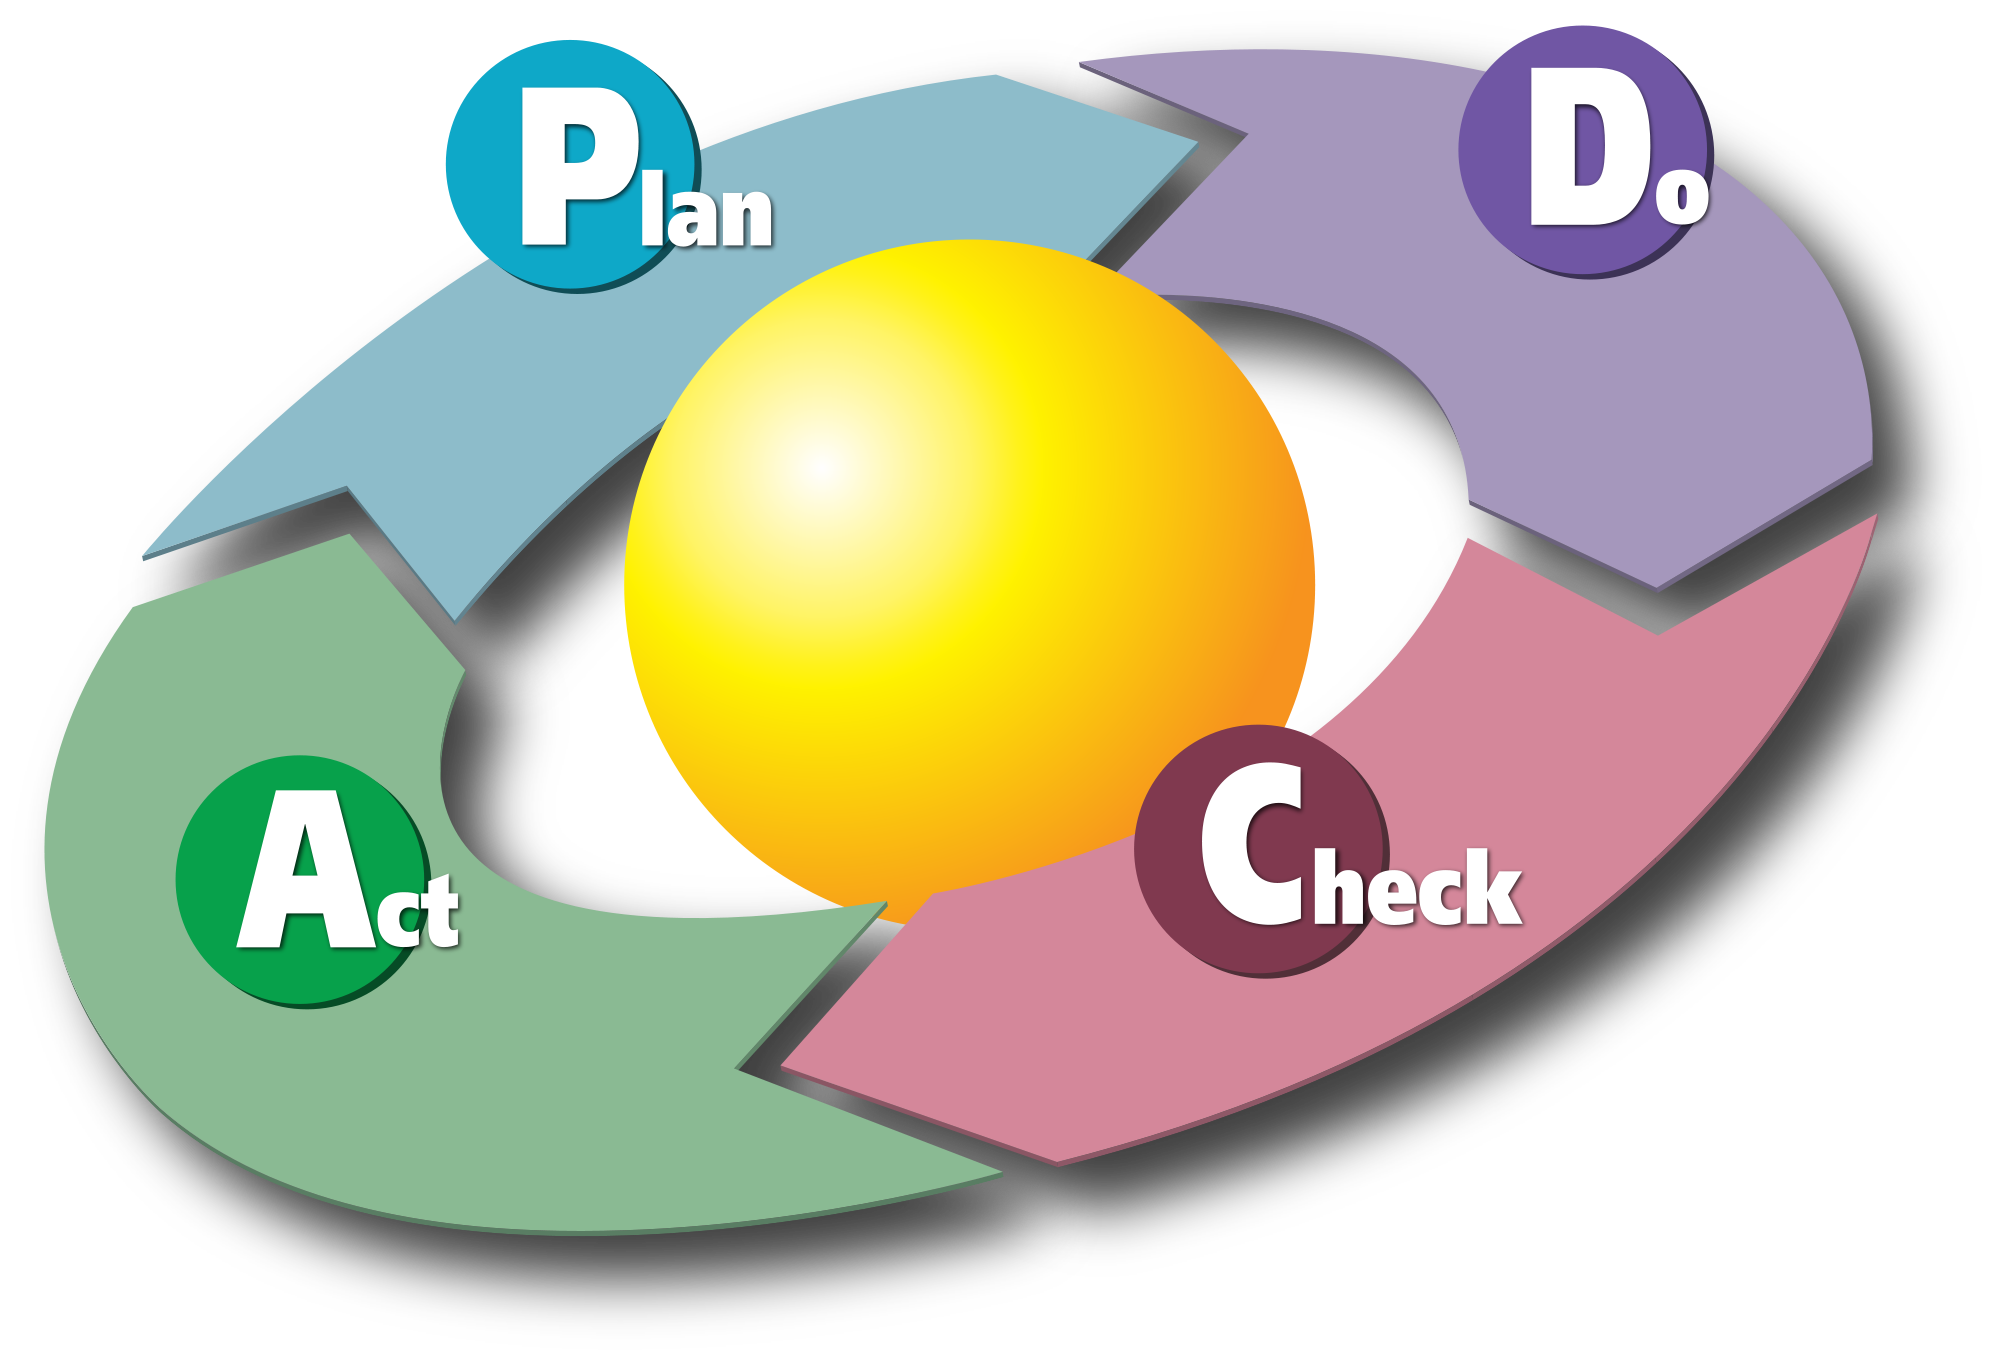
\includegraphics[scale=.2]{img/2000px-PDCA_Cycle.png}
	\caption{Modello PDCA}
	\label{fig:ModelloPDCA}
\end{figure}

Le Procedure di controllo di qualità di processo si basano sul ciclo di Deming o PDCA$_G$. Questo garantisce un miglioramento continuo di tutti i processi e delle attività di verifica che si realizza con comunicazioni attive delle componenti del gruppo e con la connessione delle fasi di analisi, progettazione, verifica e collaudo. La qualità dei processi viene monitorata anche grazie alla qualità di prodotto perché un prodotto di bassa qualità può indicare che uno o più processi vadano migliorati. Per questo motivo si presta attenzione a monitorare i singoli processi ed è necessario quindi che i processi vengano pianificati nel dettaglio, le risorse vengano ripartite nella pianificazione in modo chiaro e ci sia un adeguato controllo sui processi.


